\chapter{Stato dell'Arte}\label{chap:riferimentiStrotici}

%\section{Introduzione} \label{sec:riferimentiStorici}
%Cosa posso inserire?

\section{BlockSci} \label{sec:riferimentiStorici}

BlockSci \cite{DBLP:journals/corr/abs-1709-02489} è un sistema open source, scritto in C++, per l'analisi di blockchain basate sull'organizzazione dati di Bitcoin. Sviluppato dall'Università di Princeton, BlockSci estrae i dati dalla blockchain di Bitcoin attraverso l'utilizzo del framework RPC di Bitcoin e di un parser per l'analisi delle informazioni serializzate dal nodo Bitcoin; i dati estratti vengono salvati in flat-file e interrogati attraverso SQLite.
BlockSci, inoltre, offre un sofisticato sistema per l'analisi dei dati estratti con cui si ha la possibilità di implementare e applicare algoritmi di analisi sulla rete Bitcoin.

In questa sezione ci concentreremo  solo sul modulo relativo al parser e sull'organizzazione delle informazioni estratte. Il parser di BlockSci legge le informazioni della blockchain sequenzialmente e, durante la lettura, applica  una serie di ottimizzazioni per il corretto funzionamento del modulo di analisi.
Il risultato della scansione sequenziale dei blocchi è un grafo delle transazioni minimale; il grafo è memorizzato in una singola tabella sequenziale, le cui entry hanno il formato mostrato in Tabella \ref{tab:blockSciSerialization}.

\begin{table}
       \centering\small
           \begin{tabular}{|c|c|}
               \hline
                 \multicolumn{2}{|c|}{\textbf{Transaction}} \\
                 %\cmidrule(lr){1-2}
                 \hline
                 \multicolumn{1}{|c|}{Size} & \multicolumn{1}{c|}{Description} \\
               \hline \hline
               32 bit & Size   \\
               \hline
               32 bit & LockTime \\
               \hline
               16 bit & Input count \\
               \hline
               16 bit & Output count \\
               \hline
               128 bits each & Outputs \\
               \hline
               128 bits each & Inputs \\
               \hline
       \end{tabular}
       \caption{Struttura delle transazioni in BlockSci per la costruzione del grafo delle transazioni \cite{DBLP:journals/corr/abs-1709-02489}.\label{tab:blockSciSerialization}}
   \end{table}

In  \cite{DBLP:journals/corr/abs-1709-02489} Kalodner et al. descrivono i risultati di alcuni test relativi all'efficienza del parser; in tali test, il parser ha impiegato all'incirca 11 ore per effettuare l'estrazione dei dati dalla blockchain di Bitcoin\footnote{Tali risultati fanno riferimento alla dimensione della blockchain assunta nell'agosto del 2017: 478,559 blocchi e 140 GB di spazio totale.}; aumentando la dimensione della memoria allocata a BlockSci si possono ottenere prestazioni migliori.

\section{BiVA} \label{sec:biva}

BiVA (Bitcoin Network Visualization \& Analysis) è un software sviluppato dall'Università di Singapore che utilizza Neo4J \cite{neo4j} per la costruzione di un grafo di address attraverso l'estrapolazione dei dati tramite il framework RPC di Bitcoin-core; esso, inoltre, implementa un algoritmo di analisi su grafo per la ricerca degli address più utilizzati all'interno della blockchain di Bitcoin.\\
In \cite{DBLP:conf/icdm/OggierPD18} Oggier et al. descrivono prevalentemente l'algoritmo di analisi utilizzato e non riportano dettagli sull'implementazione né risultati sperimentali relativi all'estrazione dei dati; tuttavia, poiché il framework RPC non è progettato  per l'estrazione completa dei dati dalla blockchain, le tempistiche dovrebbero essere abbastanza elevate utilizzando un software \emph{single thread}.\\
Una porzione di grafo prodotto attraverso BiVA è rappresentata in Figura \ref{fig:bivaGraph}.

\begin{figure}
\centering
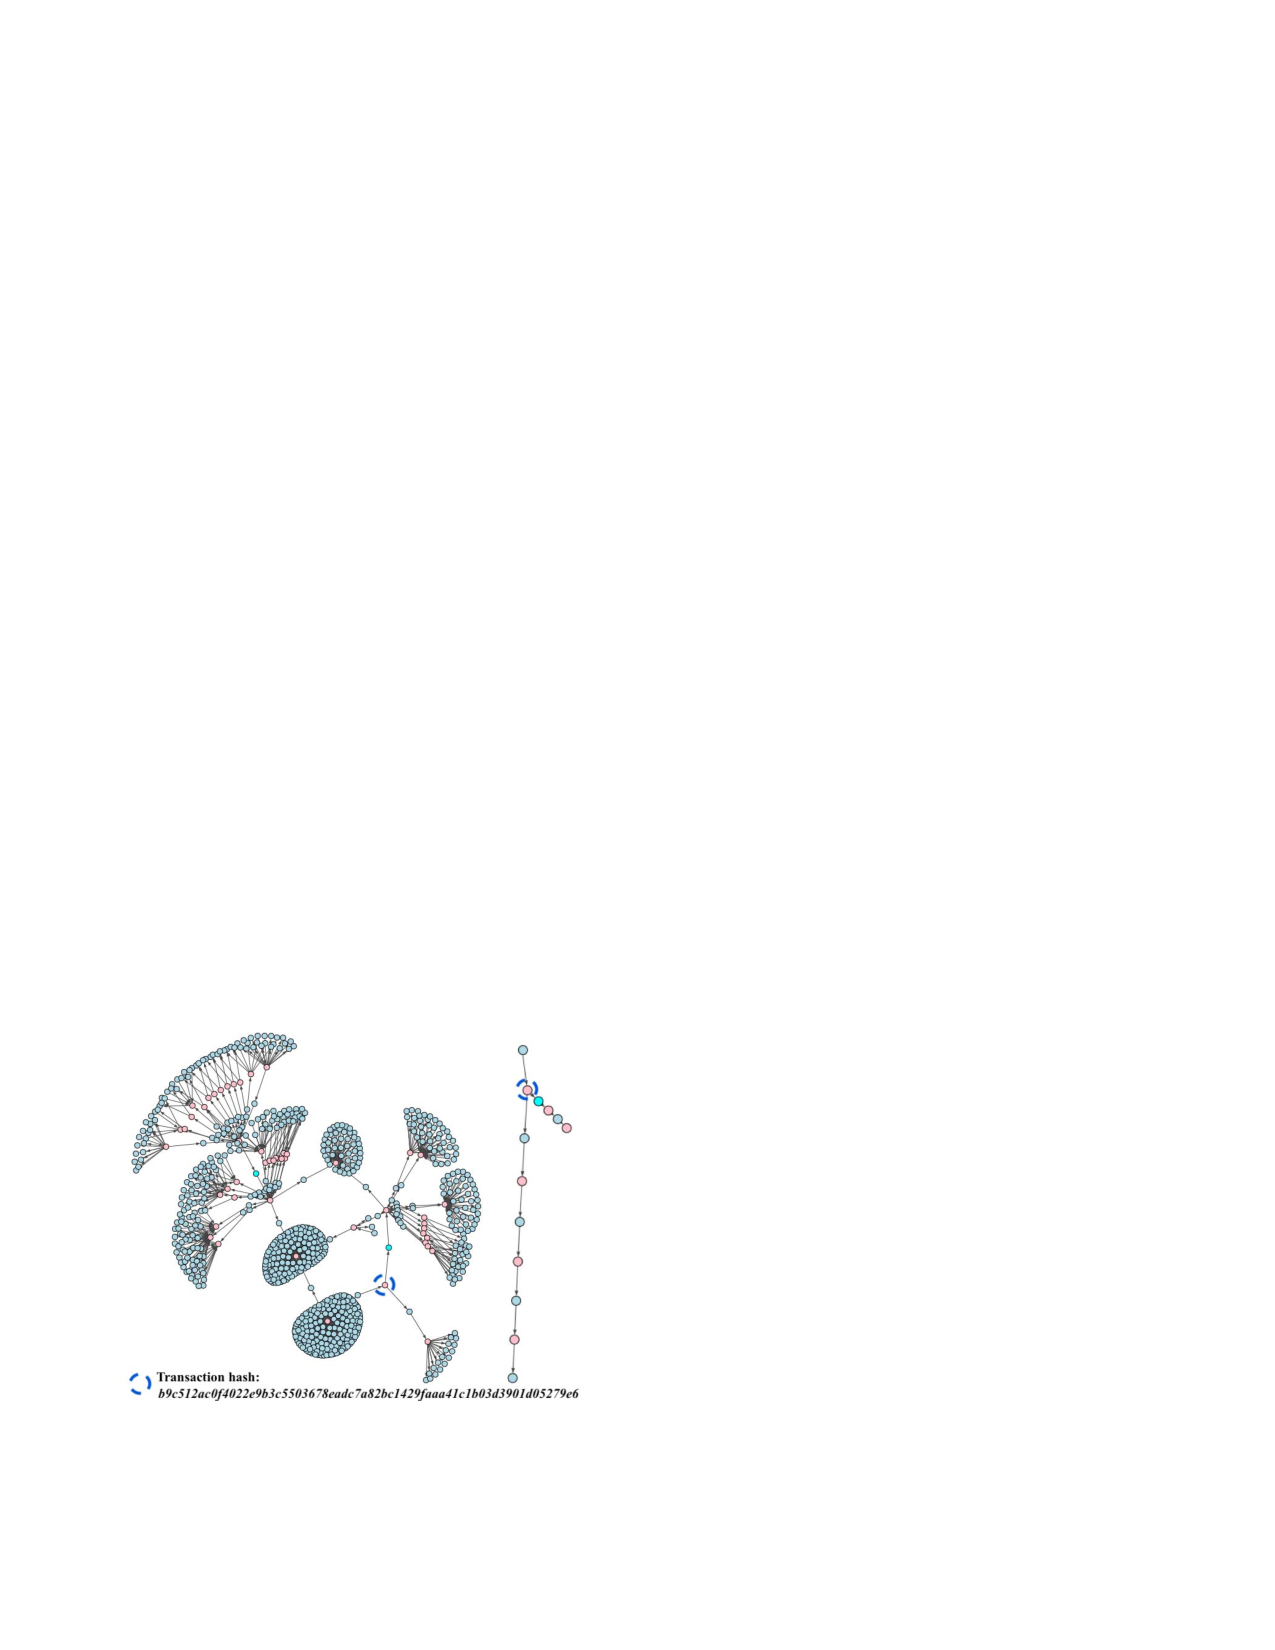
\includegraphics[scale=1.0]{images/bivaGraph.pdf}
\caption{Frammento del grafo degli address creato attraverso BiVA \cite{DBLP:conf/icdm/OggierPD18}.\label{fig:bivaGraph}}
\end{figure}


\section{Bitcoin Transaction Visualization} \label{sec:bitcoinTransactionVis}

Uno studio condotto dall'Universita di Saskatchewan e pubblicato in \cite{inproceedings} descrive la creazione di un grafo di transazioni, localizzato attraverso l'utilizzo delle API di \url{https://blockchain.com}.\\
L'utilizzo di queste API ha permesso di localizzare le transazioni, attraverso la loro posizione geografica, grazie all'IP messo a disposizione per ogni transazione. Infatti \url{https://blockchain.com} arricchisce le informazioni estratte dalla blockchain di Bitcoin, aggiungendo informazioni circa il luogo di origine della transazione; quando questa informazione non è presente, verrà utilizzata la posizione dell'Universita di Saskatchewan.
La demo per la dimostrazione di questo studio viene sviluppata attraverso tecnologie web, con un uso estensivo di JQuery. La Figura \ref{fig:bitcoinTransactionVis} ne rappresenta un esempio.

\begin{figure}[H]
\centering
\includegraphics[scale=0.1]{images/vs_article.pdf}
\caption{Frammento del grafo di transazioni prodotto attraverso la demo pubblicata nell'articolo \cite{inproceedings}.\label{fig:bitcoinTransactionVis}}
\end{figure}
